% =====================================================================
% convention.tex -- the EXOZIPPy microlensing conventions section.
%
% A drop-in \section for the EXOZIPPy microlensing paper.  \input it from
% the paper's body and run bibtex against src/exozippy/latex/references.bib
% (the universal library this repository ships); every key cited below has
% an entry there.
%
% PREAMBLE REQUIREMENTS: aastex (or any class providing \citep/\citet and
% the usual AAS journal macros), plus ONE extra line --
%
%     \usepackage{tikz}
%
% -- used only by Figure~\ref{fig:skyframe}.  Delete that one figure
% environment and the file needs nothing beyond the class itself.  No
% macros are defined here.
%
% THIS FILE IS ONE OF A PAIR.  Its twin,
% src/exozippy/components/mulensing/conventions.md, is the normative
% developer-facing list: it carries the SAME numbered claims C1-C23, and
% names for each one the source file that implements it and the test that
% pins it.  A claim may be reworded in either file, but a C-number must
% mean the same thing in both, and a claim added to one must be added to
% the other under the same number.  Keep them in one commit.
% =====================================================================

\section{Conventions}
\label{sec:conventions}

Microlensing solutions are notoriously difficult to compare across papers,
not because the physics is in dispute but because the sign and origin
conventions are.  \citet{Gould:2000} proposed a standard notation for
exactly this reason, and \citet{Skowron:2011} extended it in their
Appendix~A with the explicit goal of providing a \emph{reference} system:
even authors who do not adopt it can state how their system differs, and
solutions then translate.  We take them at their word.  This section states
every convention EXOZIPPy uses, in the form ``here is the rule, here is the
transformation to the systems you are likely to be reading''.  Each rule
carries an identifier \texttt{C}$n$; the same identifiers label the
machine-checkable version of this list distributed with the code, where
each is tied to the routine that implements it and the regression test that
pins it.

\subsection{The sky-plane frame}
\label{sec:conv:frame}

\paragraph{C1 --- the axes.}  EXOZIPPy uses the century-old astrometric
labelling throughout: $+X$ is North, $+Y$ is East, and $+Z$ is distance,
growing \emph{away} from the observer.  As a set of physical directions
this triple is left-handed, $\hat{X}\times\hat{Y} = -\hat{Z}$, and that is
deliberate rather than an oversight.  It is the only labelling that
simultaneously satisfies the textbook definitions of the Keplerian elements
and preserves the standard Euler application $R_z(\Omega)\,R_x(i)\,
R_z(\omega)$: with these axes, $\Omega$ emerges as the position angle of
the ascending node measured East of North, $\omega$ is the argument of
periastron of the orbit it names, and $\dot{Z}$ is the radial velocity with
the conventional sign (positive means receding).  Any right-handed
relabelling breaks one of the three, which is the mechanism by which this
convention has been repeatedly mangled in the exoplanet literature.

\paragraph{C2 --- the positive sense of rotation is North through East.}
Every angle on the sky in this work --- position angles, $\Omega$, the
parallax direction $\phi_\pi$, and the binary orientation $\alpha$ ---
increases from North toward East.  Drawn with North up and East to the
left, which is how we plot the sky throughout, that sense is
counterclockwise (Figure~\ref{fig:skyframe}).  This is the same statement
as \citeauthor{Skowron:2011}'s ``all coordinate systems are right-handed
\ldots\ (N,E)'': the two-dimensional pair $(\hat{N},\hat{E})$ is
right-handed even though the three-dimensional triple of C1 is not, because
the two statements are about different spaces.

\paragraph{C3 --- the basis.}  For an event at $(\alpha_{2000},
\delta_{2000})$ the sky-plane unit vectors are the spherical tangent basis
in ICRS/J2000 equatorial coordinates,
\begin{eqnarray}
  \hat{e} &=& (-\sin\alpha_{2000},\; \cos\alpha_{2000},\; 0), \\
  \hat{n} &=& (-\sin\delta_{2000}\cos\alpha_{2000}, \nonumber \\
          & & \phantom{(}
               -\sin\delta_{2000}\sin\alpha_{2000},\;
                \cos\delta_{2000}).
\end{eqnarray}
This is the basis \texttt{MulensModel} \citep{Poleski:2019} constructs as
$\hat{e} = \widehat{\hat{z}\times\hat{u}}$, $\hat{n} = \hat{u}\times\hat{e}$,
to within one unit in the last place, so the two magnification back ends we
use share a line of sight by construction rather than by coincidence.  A
single routine owns this projection; nothing in the code re-derives it at a
call site.

\begin{figure}
\centering
% Requires \usepackage{tikz}.  Delete this environment if that is
% unavailable; nothing else in this file needs it.
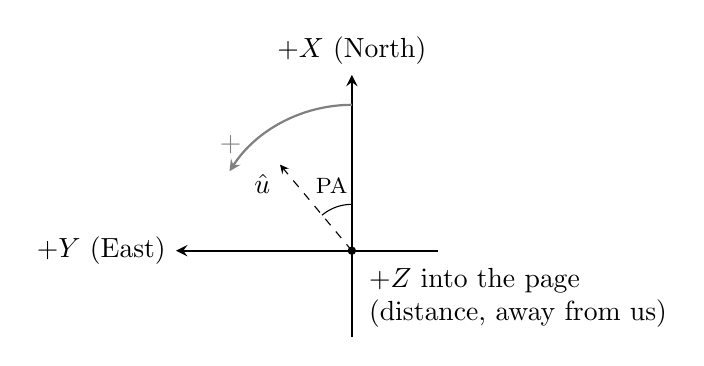
\begin{tikzpicture}[>=stealth, scale=0.95]
  % axes: North up, East to the LEFT, line of sight into the page
  \draw[->, thick] (0,-1.15) -- (0,2.35) node[above] {$+X$ (North)};
  \draw[->, thick] (1.15,0) -- (-2.35,0) node[left] {$+Y$ (East)};
  \fill (0,0) circle (1.6pt);
  \node[below right, align=left] at (0.10,-0.10)
       {$+Z$ into the page\\(distance, away from us)};
  % the positive sense: North through East, counterclockwise as drawn
  \draw[->, thick, gray] (0,1.95)
       arc[start angle=90, end angle=147, radius=1.95];
  \node[gray] at (-1.62,1.42) {$+$};
  % an example position angle, measured from North toward East
  \draw[->, dashed] (0,0) -- (-0.96,1.15) node[below left] {$\hat{u}$};
  \draw (0,0.62) arc[start angle=90, end angle=130, radius=0.62];
  \node at (-0.27,0.86) {\footnotesize $\mathrm{PA}$};
\end{tikzpicture}
\caption{The sky-plane frame (C1--C3), drawn as we plot it: North up, East
to the left, and the line of sight $+Z$ into the page, growing away from
the observer.  The triple is left-handed as a set of physical directions,
$\hat{X}\times\hat{Y} = -\hat{Z}$.  Position angles, $\Omega$, $\phi_\pi$
and $\alpha$ all increase in the sense marked $+$, from North toward East,
which is counterclockwise in this projection; the dashed ray shows a
direction $\hat{u}$ at position angle $\mathrm{PA}$.}
\label{fig:skyframe}
\end{figure}

\subsection{Origins, epochs, and the geocentric frame}
\label{sec:conv:origins}

\paragraph{C4 --- times.}  All epochs are ${\rm BJD}_{\rm TDB}$.  Light
curves supplied in another time system are converted on ingest.

\paragraph{C5 --- the geocentric frame.}  We adopt the now-standard
geocentric framework \citep{An:2002, Gould:2004}: parameters are measured in
the inertial frame moving with Earth's position \emph{and} velocity at a
fiducial epoch $t_{0,\rm par}$, in the sense of \citet{Skowron:2011}.
$t_{0,\rm par}$ is a stated configuration choice, never a fitted parameter.
The Einstein crossing time $t_{\rm E}$ and the \emph{direction} of the
parallax vector depend on it; $|\pi_{\rm E}|$, $\theta_{\rm E}$, $s$, $q$
and $\rho$ do not.  Because a stellar proper motion is a barycentric
observable while the light curve is not, EXOZIPPy applies the
\citet{Gould:2004} conversion
\begin{equation}
  \mu_{\rm rel,geo} = \mu_{\rm rel,helio}
    - \pi_{\rm rel}\, \frac{v_{\oplus,\perp}(t_{0,\rm par})}{{\rm AU}}
  \label{eq:mugeo}
\end{equation}
internally, so that a prior placed on a measured proper motion and the
$t_{\rm E}$ that enters the light curve are consistent by construction.

\paragraph{C6 --- observer positions.}  Every observer's position enters as
its \emph{deviation} from the linear reference trajectory that defines the
frame,
\begin{equation}
  \vec{\delta}(t) = \mathbf{r}_{\rm obs}(t)
    - \left[\mathbf{r}_\oplus(t_{0,\rm par})
      + \mathbf{v}_\oplus(t_{0,\rm par})\,(t - t_{0,\rm par})\right],
  \label{eq:deviation}
\end{equation}
in AU.  Ground-based observatories and spacecraft are handled by the same
expression; a satellite is simply an observatory whose deviation is of order
$1\,{\rm AU}$ rather than of order $0.003\,{\rm AU}$
\citep[cf.][Section~3]{Yee:2015}.  Zero deviations mean no parallax.

\paragraph{C7 --- relative motion is the lens relative to the source.}
Following \citet[Appendix~A.6]{Skowron:2011}, every relative quantity is
defined by the motion of the lens with the source held fixed:
$\vec{\mu}_{\rm rel} = \vec{\mu}_{\rm L} -
\vec{\mu}_{\rm S}$ and $\pi_{\rm rel} = \pi_{\rm L} - \pi_{\rm S}$.

\subsection{The source trajectory and the sign of the parallax}
\label{sec:conv:trajectory}

\paragraph{C8 --- the parallax vector.}  The microlens parallax is
\begin{eqnarray}
  \vec{\pi}_{\rm E} &=& (\pi_{\rm E,N}, \pi_{\rm E,E})
    = \frac{\pi_{\rm rel}}{\theta_{\rm E}}\,
      \hat{\mu}_{\rm rel,geo},
      \label{eq:pie} \\
  \phi_\pi &\equiv& \mathrm{atan2}(\pi_{\rm E,E}, \pi_{\rm E,N}),
  \label{eq:phipi}
\end{eqnarray}
so that $\phi_\pi$ is the position angle, East of North, of the lens's
motion relative to the source --- \citeauthor{Skowron:2011}'s definition
unchanged.  The direction is geocentric, per Equation~(\ref{eq:mugeo}).

\paragraph{C9 --- the trajectory.}  Let $\hat{\tau} =
\hat{\mu}_{\rm rel,geo}$ and let $\hat{\beta}$ be $\hat{\tau}$
rotated by $+90^\circ$ in the East-of-North sense of C2.  The angular
separation of the lens from the source, in units of $\theta_{\rm E}$, is
\begin{equation}
  \vec{u}(t) = u_0\,\hat{\beta}
    + \frac{t - t_0}{t_{\rm E}}\,\hat{\tau}
    - \frac{\pi_{\rm rel}}{\theta_{\rm E}}\,\vec{\delta}(t),
  \label{eq:traj}
\end{equation}
with $\vec{\delta}$ from Equation~(\ref{eq:deviation}) projected onto
the sky-plane basis of C3.  Two things follow.  First, because $u_0$
multiplies $\hat{\beta}$, \emph{$u_0 > 0$ means the lens passes the source
on the lens's right}, which is again \citeauthor{Skowron:2011}'s rule.
Second, the point-lens magnification \citep{Paczynski:1986} depends only on
$|\vec{u}|$, so the sign of $u_0$ is observable only through the
parallax term; see C23.

\paragraph{C10 --- the parallax signs, written out both ways.}  This is the
item most often garbled, and the difficulty is not the physics but the
symbol.  Two different sky-plane vectors are called ``$\delta$'' in the
literature, and they are exact negatives of one another (C11).  We therefore
give both displays.  Writing $(\delta_N, \delta_E)$ for the
\emph{observer's own} projected offset, Equation~(\ref{eq:deviation})
dotted into $(\hat{n}, \hat{e})$,
\begin{eqnarray}
  \tau(t) &=& \frac{t-t_0}{t_{\rm E}}
              - \delta_N\,\pi_{\rm E,N} - \delta_E\,\pi_{\rm E,E},
              \label{eq:tau_obs} \\
  \beta(t) &=& u_0
              + \delta_N\,\pi_{\rm E,E} - \delta_E\,\pi_{\rm E,N},
              \label{eq:beta_obs}
\end{eqnarray}
while writing $(\Delta_N, \Delta_E) = -(\delta_N, \delta_E)$ for the
apparent displacement \emph{of the source} per unit parallax --- the
quantity \texttt{MulensModel} calls $\delta$ ---
\begin{eqnarray}
  \tau(t) &=& \frac{t-t_0}{t_{\rm E}}
              + \Delta_N\,\pi_{\rm E,N} + \Delta_E\,\pi_{\rm E,E},
              \label{eq:tau_src} \\
  \beta(t) &=& u_0
              - \Delta_N\,\pi_{\rm E,E} + \Delta_E\,\pi_{\rm E,N}.
              \label{eq:beta_src}
\end{eqnarray}
Equations~(\ref{eq:tau_obs})--(\ref{eq:beta_obs}) and
(\ref{eq:tau_src})--(\ref{eq:beta_src}) are the same equations.  A statement
of the form ``there is a minus sign on the East terms'' is therefore not
convention-free and should never be quoted without saying which offset is
meant: in the first display $\tau$ carries a minus on \emph{both}
components, in the second a plus on both.  EXOZIPPy implements
Equations~(\ref{eq:tau_obs})--(\ref{eq:beta_obs}) in its analytic
point-lens path and (\ref{eq:tau_src})--(\ref{eq:beta_src}) in its
contour-integration path \citep{Bozza:2018, Bozza:2025}, and the two agree
to $10^{-6}$ in magnification on real ephemerides, with and without a
satellite.  Both match \texttt{MulensModel} \citep{Poleski:2019}, so
published $(\pi_{\rm E,N}, \pi_{\rm E,E})$ transfer without transformation.

The distinction has teeth.  Earth's deviation over a season is
$\sim 0.003\,{\rm AU}$, so a sign error there barely moves a ground-only
fit; a Spitzer-like deviation projects to $\sim 0.125\,{\rm AU}$, where the
same error moved the magnification near peak from $1.77$ to $1.91$ in our
own testing --- an $8$ per cent error, against photometry whose scatter is
of order $0.1$ per cent, which is the whole reason for taking the
observation.  The sign is therefore effectively untestable on ground-based
data alone and immediately fatal with a satellite.

\paragraph{C11 --- the two offsets are different quantities, not different
conventions.}  An observer displaced by $\mathbf{R}$ sees a source at
distance $d$ displaced by $-\mathbf{R}/d$.  The observer's own projected
offset and the apparent displacement of the source are therefore exact
negatives, and a code that computes both --- as any code fitting
microlensing \emph{and} astrometry must --- will appear to carry two
incompatible sign conventions when it in fact carries one convention and two
quantities.  We define one and negate it to obtain the other.

\subsection{Binary and multiple lenses}
\label{sec:conv:binary}

\paragraph{C12 --- the origin is the lens centre of mass.}
\citet{Skowron:2011} require the ``system centre'' defining $t_0$ and $u_0$
to be stated; ours is the centre of mass of all lens bodies, evaluated at
$t_{0,\rm par}$.

\paragraph{C13 --- lengths are in Einstein radii of the total lens mass.}
$\theta_{\rm E}^2 = \kappa\, M_{\rm L,tot}\, \pi_{\rm rel}$, and
$t_{\rm E}$, $\rho$, $s$ and $\pi_{\rm E}$ all inherit that normalisation,
for any number of lens bodies.  The sampled separation coordinate is
$\log_{10} s$, which renders the close/wide degeneracy the exact reflection
$\log_{10} s \rightarrow -\log_{10} s$.

\paragraph{C14 --- $q$, and why $q > 1$ is permitted.}  The mass ratio is
$q_j = M_j / M_1$ for each companion $j$, where body $1$ is whichever body
the configuration lists \emph{first}.  ``Primary'' is thus a slot label, not
a claim about which body is heavier, and EXOZIPPy imposes no $q \le 1$
restriction: the lens with the labels exchanged is the same physical system
(C19), and the magnification algorithms are indifferent.  This matters when
seeding from the literature, where the near-universal habit of naming the
heavier body the primary means a published $q$ may need inverting.  Our fit
to OGLE-2016-BLG-1003, a binary-source binary-lens event, carries
$q = 1.19$ directly as \citet{Jung:2017} report it.

\paragraph{C15 --- $\alpha$.}  For each companion $j$, $\alpha_j$ is the
angle from the primary-to-companion-$j$ axis to the direction of
lens-source relative motion $\hat{\tau}$, measured counterclockwise in the
sense of C2.  Equivalently, in the trajectory frame whose $+x$ axis is
$\hat{\tau}$ and whose $+y$ axis is $\hat{\beta}$, with the origin at the
lens centre of mass, the source sits at $(-\tau, -\beta)$ and companion $j$
at $s_j(\cos\alpha_j,\, -\sin\alpha_j)$ relative to the primary.  Every
companion's angle is measured from the same $\hat{\tau}$, so an $N$-body
lens has $N-1$ independent orientations and no chained angles.

Note that the source \emph{moves} along $-\hat{\tau}$: $\hat{\tau}$ is the
direction in which the lens moves relative to the source.  Measuring
$\alpha$ to the source's own direction of travel instead --- an easy reading
of the phrase ``the source trajectory angle'' --- differs by exactly
$180^\circ$, and is the commonest single cause of an $\alpha$ that will not
reproduce a published light curve (C21).

\paragraph{C16 --- how $\alpha$ is sampled.}  $\alpha$ is not sampled
directly.  We sample an unconstrained Cartesian pair
$(x_\alpha, y_\alpha)$ and take $\alpha = \mathrm{atan2}(y_\alpha, x_\alpha)$, so
the angle has no periodic boundary for the sampler to stall against.  This
is a parameterisation choice and not a convention: the reported $\alpha$
means C15.

\paragraph{C24 --- lens orbital motion.}  In the linear mode the companion
geometry evolves as
\begin{equation}
s_j(t) = s_{j,0} + \dot{s}_j\,(t - t_{0,\rm par}), \qquad
\alpha_j(t) = \alpha_{j,0} + \dot{\alpha}_j\,(t - t_{0,\rm par}),
\end{equation}
with both rates constant, anchored at the same fiducial epoch
$t_{0,\rm par}$ the parallax uses (C5) --- the shared anchor, recommended by
\citet{Skowron:2011} (their Eq.~A17), is what makes the orbital and parallax
terms composable.  These definitions are those of \texttt{MulensModel} (the
identity mapping of C18 extends to $\dot{s}$ and $\dot{\alpha}$) and of
\citet{Skowron:2011} Section~3.3.1 up to one sign of vocabulary: their
velocity components $(\gamma_\parallel, \gamma_\perp)$ --- parallel and
perpendicular to the binary axis, a right-handed pair oriented like
$(N, E)$ --- satisfy
\begin{equation}
\gamma_\parallel = \dot{s}/s_0, \qquad
\gamma_\perp = -\dot{\alpha} = +\frac{d\,\mathrm{PA_{axis}}}{dt},
\label{eq:gammaperp}
\end{equation}
their Appendix~A.4.  The minus sign is a consequence of C15 itself: $\alpha$
is measured \emph{from} the (moving) binary axis \emph{to} the fixed
$\hat{\tau}$, so it runs opposite to the axis's own position angle, and
$\gamma_\perp$ is the axis's physical sky rotation rate, positive in the C2
sense.  No handedness correction enters: our left-handed triple (C1) and
\citet{Skowron:2011}'s right-handed one differ only in which way the
line-of-sight axis points, and that flip cancels the handedness-label flip
identically in the sky plane.  A sign for $\dot{\alpha}$ or $\gamma_\perp$
is meaningful only jointly with $\mathrm{sign}(u_0)$: the orbiting-binary
ecliptic degeneracy (their Eq.~A16) reverses
$(u_0, \alpha, \pi_{\rm E,\perp}, \gamma_\perp)$ together.  In the Keplerian
mode the same definitions are driven by a projected orbit,
$s_j(t) = |\vec{\delta}_j(t)|$ and $\alpha_j(t) = \alpha_{j,0} -
[\mathrm{PA_{axis}}(t) - \mathrm{PA_{axis}}(t_{0,\rm par})]$, where the
minus sign is Equation~\ref{eq:gammaperp} again; its correctness is pinned
against a synthetic orbit of known inclination rather than against a fit,
because the rotation sense of the binary axis is the only quantity here
that measures $\mathrm{sign}(\cos i)$, and the wrong sign lowers no
$\chi^2$ --- it silently reports the reflected orbit
($\Omega_{\rm node} \rightarrow -\Omega_{\rm node}$,
$i \rightarrow 180^\circ - i$; their Section~5.2).

\subsection{Translating to and from other conventions}
\label{sec:conv:mappings}

Table~\ref{tab:conventions} summarises.  The entries are stated as
transformations \emph{onto} the system defined above.

\paragraph{C17 --- \citet{Skowron:2011}, Appendix~A: identity.}  All three
of that appendix's sign rules hold here unchanged --- $u_0 > 0$ when the
lens passes the source on its right, $\phi_\pi$ counterclockwise from North,
and $\alpha$ counterclockwise from the primary-secondary axis to the lens's
motion --- as do $q = M_2/M_1$, $s$ in Einstein radii, and the geocentric
$t_{0,\rm par}$ framework.  A solution reported in that reference system
transfers with no transformation whatever, which is exactly what the
appendix was written to make possible.

\paragraph{C18 --- \texttt{MulensModel}: identity, with a caveat about its
documentation.}  $t_0$, $u_0$, $t_{\rm E}$, $\rho$, $\pi_{\rm E,N}$,
$\pi_{\rm E,E}$, $t_{0,\rm par}$, $s$, $q$ and $\alpha$ all mean the same
thing in \texttt{MulensModel} \citep{Poleski:2019} as here; our
implementations are checked against it directly.  The caveat is worth
recording because it is precisely the kind of note that propagates a
$180^\circ$ error: \texttt{MulensModel}'s \texttt{Trajectory} class states
in its documentation that it follows \citeauthor{Skowron:2011}'s
Appendix~A ``except the definition of \emph{alpha}, which is shifted by
180 deg''.  Taken against what Appendix~A.6 actually says --- that
$\alpha_0$ is the angle of the \emph{lens} motion relative to the
primary-secondary axis --- the shift is not there.  With $\alpha = 0$,
\texttt{MulensModel} places the source at $+x$ before $t_0$ and $-x$ after
it, so the lens moves relative to the source from the primary toward the
secondary, which is $\alpha = 0$ in \citeauthor{Skowron:2011}'s sense.  We
follow Appendix~A as written, which is also what \texttt{MulensModel}
computes.

\paragraph{C19 --- exchanging the primary and secondary labels.}  This is a
pure relabelling; the centre of mass, the trajectory and the light curve are
untouched.  Only two parameters move:
\begin{equation}
  q \rightarrow 1/q,
  \qquad
  \alpha \rightarrow \alpha + 180^\circ,
\end{equation}
with $s$, $t_0$, $u_0$, $t_{\rm E}$, $\rho$ and $\vec{\pi}_{\rm E}$
unchanged.  This is the transformation to apply when a published $q \le 1$
belongs to the body our configuration lists second (C14).

\paragraph{C20 --- codes whose $\alpha$ is a sky position angle.}  Some
codes define the binary orientation absolutely rather than relative to the
trajectory.  \texttt{BAGLE} \citep{Bhadra:2026}, for instance, defines
$\alpha$ as the angle between North and the binary axis, incrementing
eastward.  There is no fixed offset between such an $\alpha$ and ours,
because the conversion involves the relative-motion direction and therefore
the fit itself:
\begin{equation}
  \alpha_{\rm here} = \phi_\pi - {\rm PA}(\textrm{primary}
    \rightarrow \textrm{companion}) \pmod{360^\circ},
\end{equation}
with $\phi_\pi$ from Equation~(\ref{eq:pie}).  Before applying this, confirm
which end of the axis the other code's position angle refers to; a
secondary-to-primary convention adds a further $180^\circ$.

\paragraph{C21 --- papers whose $\alpha$ is measured to the source
trajectory.}  As noted in C15 this is a $180^\circ$ shift, and composed with
the opposite $u_0$ branch (C23) it appears as the reflection-plus-shift
$\alpha \rightarrow 180^\circ - \alpha$.  Our fit to OGLE-2016-BLG-1003 is
the worked example: \citet{Jung:2017} report $\alpha = 48.243^\circ$, and the
value that reproduces their light curve in our convention is
$131.757^\circ = 180^\circ - 48.243^\circ$ with $u_0 > 0$ (its mirror partner,
$u_0 < 0$ with $\alpha = 228.243^\circ$, is the same physical solution by C23).
We stress that this is a fact about one paper's convention, established for
that event by a $\chi^2$ scan and not by assumption.  \emph{There is no
general rule.}  The reliable procedure when adopting a published solution is
to evaluate the eight combinations $(\pm u_0) \times (\alpha, -\alpha,
180^\circ \pm \alpha)$ at the published values of everything else and keep
the one the light curve prefers; seven of the eight are typically
catastrophic, and the exercise costs seconds.

\paragraph{C22 --- when no mapping exists.}  It is worth recording that the
procedure above can legitimately return nothing.  The answer key of the 2018
Roman (\textit{WFIRST}) microlensing data challenge carries an $\alpha$ for
each of the 44 events in its sample, and we were unable to map it onto the
fitted convention by \emph{any} global transformation.  We tested this
rather than assumed it: for each event we scanned $\alpha$ at the answer
key's own values of $t_0$, $u_0$, $t_{\rm E}$, $\rho$, $s$ and $q$, fitting
the fluxes linearly, to obtain the $\alpha$ the simulated light curve itself
prefers.  Against that reference, every candidate transformation --- the
difference, the reflection, either with the Galactic-to-equatorial position
angle removed, and either with ${\rm PA}(\mu_{\rm rel})$ removed, i.e.\ the
hypothesis that the key uses a position-angle $\alpha$ in the sense of C20
--- scatters like noise, with circular concentrations $R \le 0.19$ where
$R = 1$ would mean the transformation \emph{is} the rule.  Restricting to
the twelve events whose anomaly constrains $\alpha$ most sharply does not
help ($R = 0.22$ and $0.41$, against $R \approx 0.29$ expected from twelve
random angles), so this is a property of the key rather than of a weak
constraint or of the wrong degeneracy branch.  We therefore report $\alpha$
for those events without a truth value and without a pull, in preference to
a search over candidate mappings that always returns its closest candidate
and so cannot fail visibly.  The failure mode is not hypothetical: such a
search reported a $2034\sigma$ discrepancy in $\alpha$ for one event whose
fitted value lay $0.3^\circ$ from the light curve's own optimum.

\paragraph{C23 --- the discrete degeneracies, and why signs travel in
pairs.}  For a static binary with no parallax, $(u_0, \alpha) \rightarrow
-(u_0, \alpha)$ is an exact symmetry of the light curve
\citep{Skowron:2011}, so neither the sign of $u_0$ nor the value of $\alpha$
is meaningful on its own; they can only ever be established together.  With
parallax the symmetry is broken but survives approximately as the ecliptic
degeneracy, $(u_0, \alpha, \pi_{\rm E,\perp}) \rightarrow -(u_0, \alpha,
\pi_{\rm E,\perp})$, which for bulge sources is strong \citep{Smith:2003}.
Following \citet{Skowron:2011} we reserve $u_0 < 0$ for solutions that
include parallax.  We note that our numerical floor on $|u_0|$ preserves its
sign, precisely so that the first of these symmetries remains exact within
the implementation.

\begin{table*}
\centering
\caption{Transformations onto the conventions of
Section~\ref{sec:conventions}.  ``Identity'' means a published value may be
adopted unchanged; a dash means the source system agrees, or says nothing.}
\label{tab:conventions}
\begin{tabular}{llll}
\hline\hline
Source system & $q$ & $\alpha$ & $u_0$, $\vec{\pi}_{\rm E}$ \\
\hline
\citet{Skowron:2011} Appendix~A (C17)         & identity & identity                        & identity \\
\texttt{MulensModel} (C18)                    & identity & identity                        & identity \\
Primary/secondary labels exchanged (C19)      & $1/q$    & $\alpha + 180^\circ$            & identity \\
$\alpha$ a sky position angle (C20)           & ---      & $\phi_\pi - \mathrm{PA_{axis}}$ & --- \\
$\alpha$ to the source trajectory (C21)       & ---      & $\alpha + 180^\circ$            & --- \\
\quad composed with the $u_0$ branch          & ---      & $180^\circ - \alpha$            & $-u_0$ \\
2018 Roman data challenge key (C22)           & identity & \textit{none exists}            & $|u_0|$ only \\
\hline
\end{tabular}
\end{table*}
